\newpage
\section{Diagrama de Interrelación de Documentos}

Una vez obtenido el diseño de la base de datos que deseamos modelar, 
el siguiente paso es comenzar a transformar dicho modelo en un esquema 
de documentos. Para ello utilizamos el Diagrama de interelacion de 
Documentos, con el objetivo de poder ilustrar como nuestro modelo 
resuelve las consultas del enunciado de forma eficiente. Para ello
iremos viendo cada consulta y trateremos de modelar los documentos 
en base a ellos.\\ \\

\subsection{Consultas}

La \textbf{primera consulta} requiere: devolver la cantidad de enfrentamientos ganados 
por competidor para un campeonato dado. Es decir, que si busco un registro 
particular de Campeonato, necesitamos poder devolver tuplas de 
$(competidor,cantidadDeEnfrentamientosGanados)$. En consecuencia, además de
contar con la lista de competidores que participaron en cada Campeonato, 
almacenaremos tambien sus cantidades de enfrentamientos ganados.\\

Para la \textbf{segunda consulta} y \textbf{tercera consulta}, se necesita poder obtener las 
cantidades de medallas pr campeonato y el total de medallas en la historia
(consultas 2.3 y 2.2 respectivamente). Usando el mismo razonamiento que en 
la consulta anterior; almacenamos un arreglo de campeonatos junto a la cantidad 
de medallas obtenidas en el mismo. Luego resolver la consulta se reduce a sumar 
todas las medallas, en el caso de la 2.2, y encontrar el maximo valor para la 
consulta 2.3. \\

El caso del punto \textbf{2.4} quedo resuelto en la etapa de diseño. Como los arbitros 
poseen una lista con sus participaciones en los campoeonatos, podemos resolver 
esta consulta fácilmente tomando el tamaño de la misma. \\ 

Para la \textbf{consulta 2.5} volvemos a interactuar con campeonatos y competidores
de forma similar a la primer consulta. La única diferencia es que ahora 
necesitamos conocer las escuelas a las cuales pertenecen los competidores.
La solución que encontramos fue la siguiente: reorganizar la lista de competidores de 
cada y agruparlos por Escuela. De esta manera, podemos contabilizar rápidamente la
cantidad de competidores por Escuela, y ademas cumplir con las consultas 2.2 y 2.3.\\

Para la \textbf{ultima consulta (2.6)} se nos pide obtener los competidores que más 
medallas obtuvieron por categoria. Para ello decidimos incluir en el $Competidor$, un 
campo por cada una de las categorias en el cual se lleve la cuenta de las 
medallas obtenidas por dicho competidor. Luego, para resolver la consulta, 
podemos recorrer la tabla de competidores y quedarnos con aquellos  que 
tengan mayor cantidad de medallas en alguna de las categorias. \\ ||

Teniendo en cuenta estas consideraciones, el diagrama de interrelación de 
Documentos resultante será:\\ \\

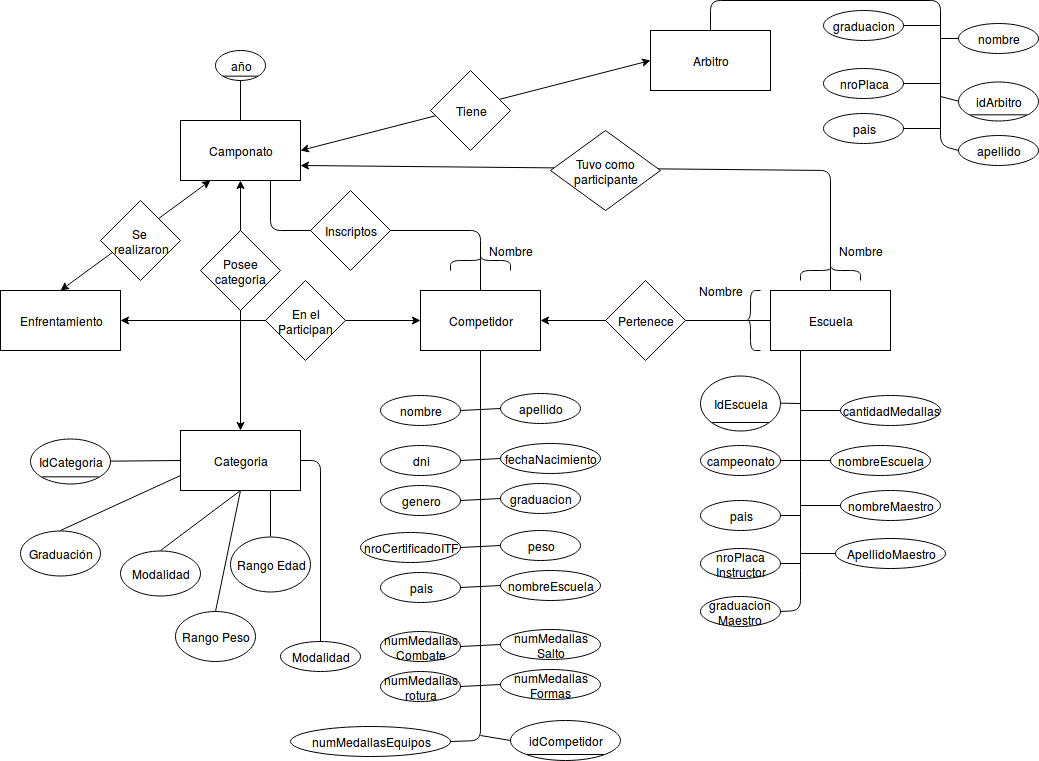
\includegraphics[angle=90,scale=0.55]{DID.png}



 


